%!TeX root = ../main.tex

\section{Conclusions}
By finishing the reconstruction in COLMAP, a final result is obtained and in this case, as shown in fig.\ref{fig:fountain}, the fountain is rebuilt in a more sparse form due to the smaller amount of information provided to the software. In fact, there is a mean observations per image equal to 4751.36 and a total number of observations equal to 52256. The data are almost a third lower than those obtained with the SURF algorithm without using the compression of the descriptors. 

\begin{figure}[h!]
    \centering
    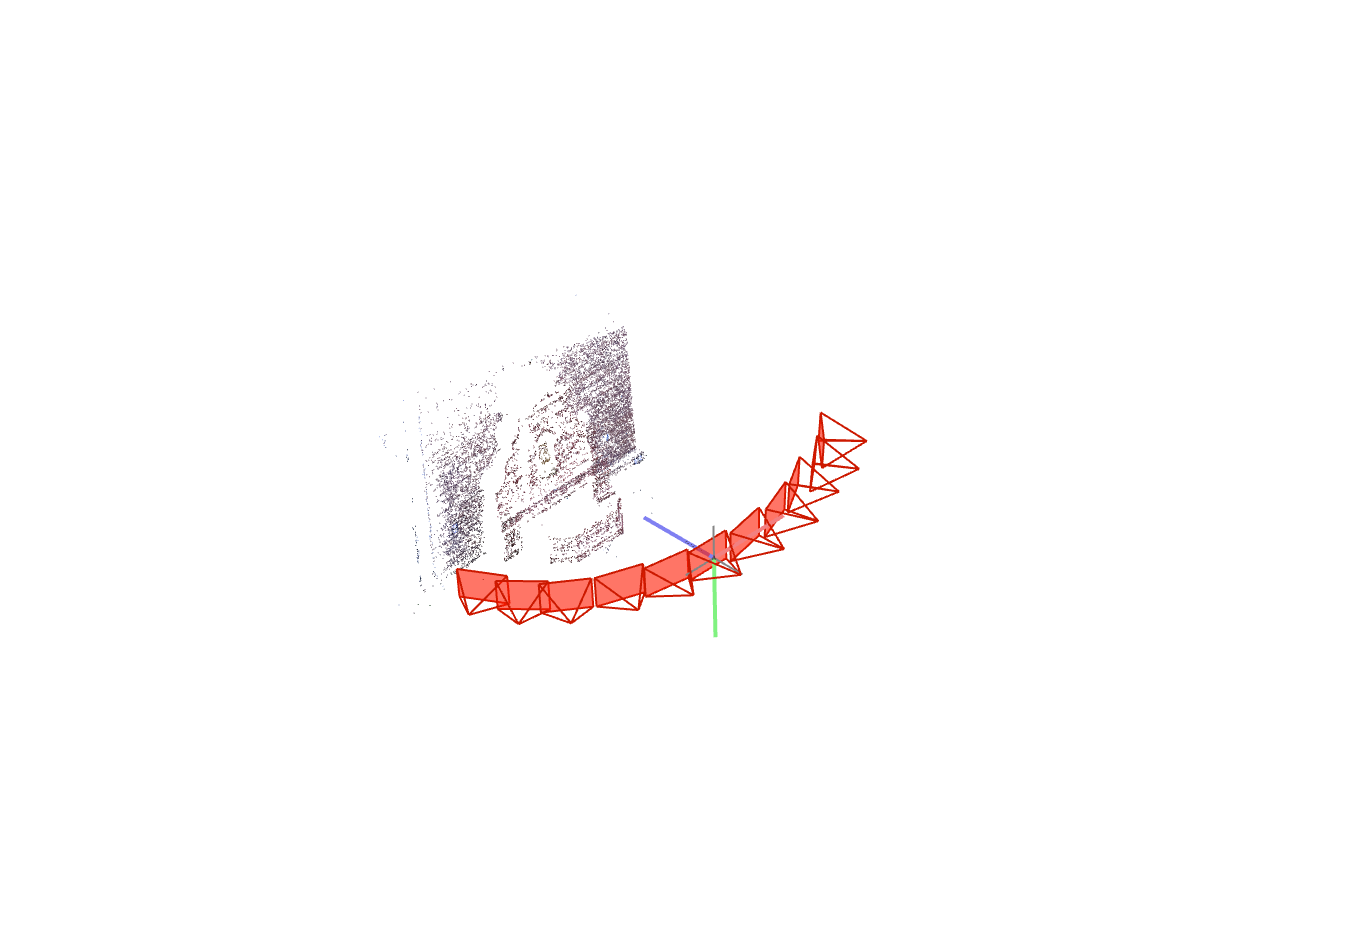
\includegraphics[width=0.7\textwidth]{images/fountain.png}
    \caption{Fountain reconstructed with the autoencoder.}
    \label{fig:fountain}    
\end{figure}

The fig.\ref{fig:fountain1} refers precisely o the final result without the use of the autoencoder and therefore all the features and matchings obtained by the SURF algorithm are supplied to COLMAP without regression. Comparing the two results a significantly differences are shown in the reconstruction quality of the fountain.

\begin{figure}[h!]
    \centering
    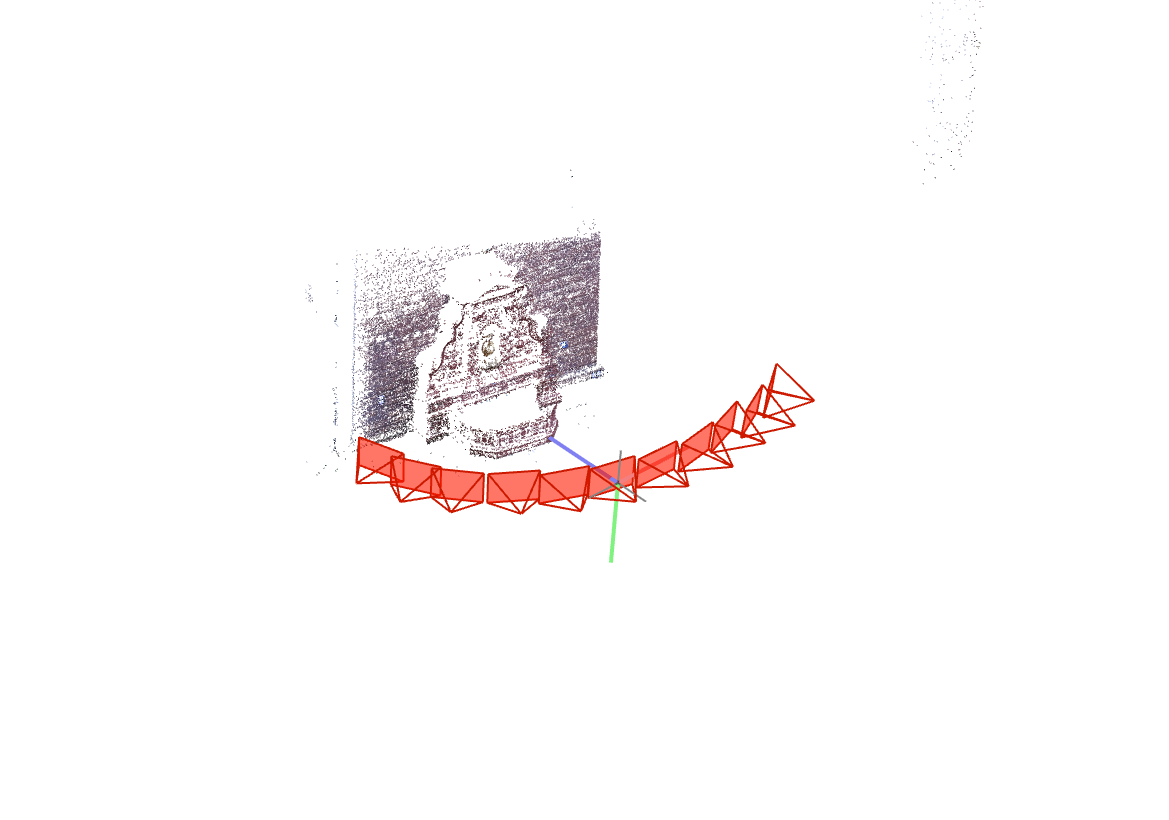
\includegraphics[width=0.7\textwidth]{images/fountain1.png}  
    \caption{Fountain reconstructed without the autoencoder.}
    \label{fig:fountain1}    
\end{figure}